\documentclass[12pt,a4paper,twoside]{ipb}

% comentar caso seja uma disseração de mestrado
% \usepackage{projei}

\usepackage[english]{babel}
\graphicspath{{./images/}}
\usepackage{listings} % incluir listagens
\usepackage{url} % typeset URL's
\usepackage[colorlinks=true,
                    urlcolor=black, %blue
                    linkcolor=black,
                    citecolor=black, %cor das citações
                    bookmarks=true,
                    pdfstartview=FitH]{hyperref}

% Pode ser usado biblatex
\usepackage[style=ieee,backend=biber]{biblatex}
\addbibresource{lib/refs.bib}

\usepackage{lipsum}

\usepackage{tabulary}

%%%%%%%%%%%%%%%%%%%%%%%%%

\title{Yabi - Yet Another Business Inteligence}

\author{Vitório Miguel Prieto Cilia - 40920}
%\authnum{1}
\secondauthor{Nome do Aluno - Número Mecanográfico}
%\secauthnum{2}

\supervisor{Prof. Albano Alves}
\cosupervisor{Prof. Lúcio Valentin}

% Para definir o ano letivo
\courseyear{2017-2018}

% Para nao mostrar a lista de tabelas
%\tablespagefalse

\makeglossaries
\loadglsentries{acronym}


%http://tex.stackexchange.com/questions/59572/custom-page-numbering-for-appendix
\usepackage{etoolbox}


\begin{document}
	
% Coloca a capa, primeira pagina e outros

\beforepreface

%\cleardoublepage

\prefacesection*{Dedicatória}
%\thispagestyle{empty}

%\lipsum[1]

(Facultativo) Dedico este trabalho a ...

%\vfill
%\pagebreak
%\mbox{}
%\vfill
%\pagebreak

%\cleardoublepage

\prefacesection*{Agradecimentos}
%\thispagestyle{empty}

%\lipsum[1]

Firstly, I would like to thank my friends Daniel Costa Valério, Henrique Pinheiro and Sávio Camacam. Together we formed the HEDANVISA group, not only sharing technical knowledge but also forming long-lasting relations.

I would like to also thank both institutions, \gls{UTFPR} and \gls{IPB} for the opportunity of realizing my masters in the scope of a double degree program.

Special thanks Professor Marcos Silvano for enabling Computer Science students of \gls{UTFPR}, Campo Mourão to apply for this program and to Bruno Mendes for his clarifying explanations in regards to writing this document.

%\vfill
%\pagebreak
%\mbox{}
%\vfill
%\pagebreak


%\cleardoublepage

\prefacesection*{Resumo}
%\thispagestyle{empty}

No contexto do Instituto Politécnico de Bragança durante o período de matrículas, o departamento de serviços informáticos é frequentemente interrompido em busca de questionamentos sobre as informações contidas nas bases de dados da instituição.

Para amenizar isso, o Yabi foi desenvolvido. Esta é uma aplicação Web construida com uma interface de usuário feita no Framework Angular e uma aplicação remota que implementa as funcionalidades necessárias e é escrita em Java com o framework Spring. De maneira geral ela fornece um portal que possibilita os colaboradoes da instituição a ter acesso as informações contidas nas bases de dados sem que seja necessário o conhecimento técnico.

Por fim, considera-se que a aplicação final atende aos requisitos de maneira suficiente para ser considerada útil e ao mesmo tempo fornece uma plataforma para desenvolvimentos futuros.

\mbox{}\linebreak
\noindent {\bf Palavras-chave:} plataforma web, business intelligence, angular, spring boot.


%\vfill
%\pagebreak
%\mbox{}
%\vfill
%\pagebreak

%\cleardoublepage

\prefacesection*{Abstract}
%\thispagestyle{empty}

Direct translation (maximum of 250 words) to English of the section ``Resumo''.

\mbox{}\linebreak
\noindent {\bf Keywords:} direct translation of ``Palavras-chave''

%\vfill
%\pagebreak
%\mbox{}
%\vfill
%%\pagebreak

% Coloca indices
\afterpreface
%\cleardoublepage
%\printglossary[type=\acronymtype,title={Acrónimos}]
\printglossary[type=\acronymtype,title={Siglas}]

\bodystart


% Capitulos do documento
\cleardoublepage
\chapter{Introduction}

\section{Textual Convetions}

\texttt{Typewritter} text is used to reference pieces of code or parts of a system, e.g. \texttt{Authentication}, \texttt{SqlQueryController}, \texttt{DatabaseReader.runQuery}, \texttt{varchar}.

\textit{Italic} \todo{mau escrito} references message passing or class methods without a corresponding parent object, e.g. \textit{authenticate}, \textit{runQuery}.

\textsl{[Slanted] - Italic}

\emph{Emphasize}

\textbf{Bold} idicates resource paths, e.g. \textbf{/user}, \textbf{/PermissionTrees}, \textbf{/runQuery/\{id\}}.

\textsc{small caps} are used to denote HTTP verbs, e.g. \textsc{delete}, \textsc{get}.

\textsf{Sans Serif}

\textrm{Roman}

\cleardoublepage



\cleardoublepage
\chapter{objective}

\cleardoublepage
\input{chapters/concepts_and_technologies}
\cleardoublepage
\chapter{Project}
This section will discuss the entities and requirements evaluated from the proposal.

\section{Requirements}
From the written proposal, some requirement were evaluated:
\begin{enumerate}
\item The system should be able to run queries in the database currently employed at the institution.\label{req:multidb}
\item Users can only run queries in which they have Permission to.\label{req:permission}
\item Query commands may be longer than 30 lines long.\label{req:longquery}
\item Running a Query yields a table that can be downloaded.\label{req:download}
\item No \gls{SQL} knowledge is needed to execute a Query.\label{req:noknowledge}
\item The system enables the insertion of new Queries.\label{req:addquery}\todo{dependendo do perfil do utilizador??}
\end{enumerate}

Given the context and the objective of this project, four entities were found to play a significant role:
\begin{description}
\item[Database]
  Where a Query is run.
\item[Query]
  A script that is run in a Database and gather information into a single table.
\item[Permission]
  The binding between Users and Queries.
\item[User]
  Either an user or an Administrator that interacts with the system.
\end{description}

Use cases were also identified:
\begin{description}
\item[User]
  \begin{enumerate}
  \item Execute a query
  \end{enumerate}
\item[Administrator]
  \begin{enumerate}
  \item \gls{CRUD} Query
  \item \gls{CRUD} Permission
  \item \gls{CRUD} Directory
  \item Associate User and Permission
  \end{enumerate}
\end{description}

\todo{importante mas nao sei onde por ainda}
Queries must be associated to one Permission.
Users may have more than one permission.
The system must authenticate using the institute's centralized directory server.
An Administrator can manage the system by altering everything that is in the scope of this system.

Permissions is a central piece of this system. It's what associates users with information.
Permissions follow a hierarchy. There is a root Permission whose path is simply ``/'' and it's parent is itself.
There are two roles that any given user may be assigned to, either Administrator or User.

\section{Class Diagram}
\todo{de alguma forma, chegou nesse diagrama}
\begin{figure}
  \centering
  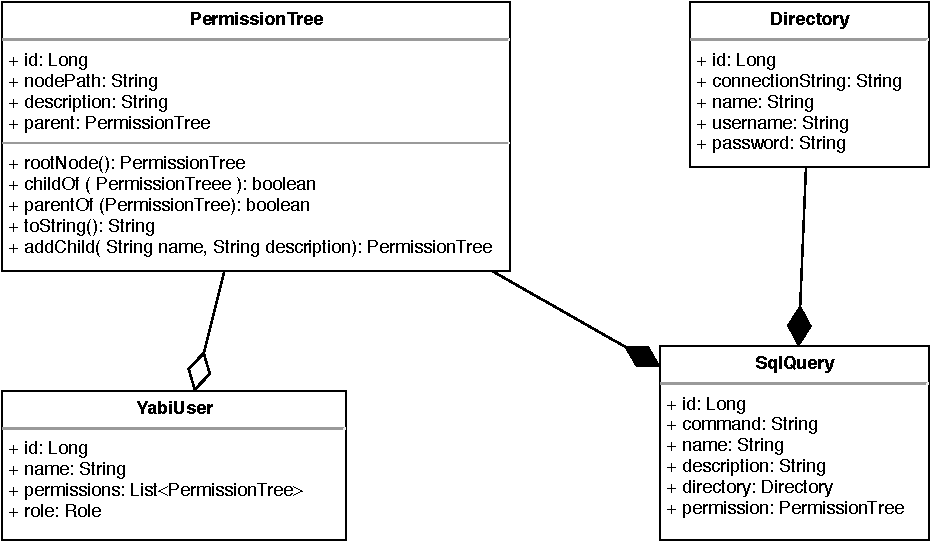
\includegraphics[width=.5\textwidth]{images/diagramas/class}
  \caption{Class diagram}\label{fig:classdiagram}
\end{figure}

\section{Template Sb-Admin-Material}
\section{Multi-Database Support}

Even though the context in which the application described in this document will be primarily accessing Oracle databases, support for other databases was added to broaden its usefulness.

As far as the project for implementing this feature goes, Figure\ref{fig:multidbproj} hopefully describes the process. When a request to run a given Query arrives,

\cleardoublepage
\input{chapters/implementation_and_results}
\cleardoublepage
\chapter{Conclusion}

With the growing adoption of digital processes by companies and institutions, the access to information becomes less available to the general public and more focused to experts in the field. These experts then end up mediating the interaction between those who are part of the decision-making process and the information storage.

Being in this situation, \gls{IPB}'s \gls{IT} department is often interrupted form their daily tasks to handle the most diverse inquiry and questions about the institution's data base.

The present system is designed to aid everyone that takes part in this process as it is able to provide int a efficient and organized manner digital information without the need for much technical knowledge, which in turn lowers the amount of daily interruptions in the \gls{IT} department.
% end of recapitulacao
% capacidades
It currently achieves this by providing a web interface in which the institution members can login, choose one of the many inquiries registered by the \gls{IT} department and download its results, lowering the amount of daily interruptions.

% o que ficou ruim
In the end, some functionalities were not implemented. The most missed one is the ability for the users to tweak their inquiries to similar but specific needs.
% O que ficou bom
In spite of this the final system accomplishes the main task of providing users with the most used inquiries provided that the \gls{IT} department registers them. Not only providing the inquiries, it also supplies the necessary tools to manage users, permissions and remote databases, all through a web interface.
\cleardoublepage
\input{chapters/future_work}

%% estilo de referências. outros valores posíveis são 'plain' e 'abbrv' apalike
%\bibliographystyle{plain}
%% listagem de referências
%\bibliography{lib/refs}

%  Caso seja usado biblatex
\printbibliography


% Apêndices
\appendix

%http://tex.stackexchange.com/questions/59572/custom-page-numbering-for-appendix
\pretocmd{\chapter}{%
	\clearpage
	\pagenumbering{arabic}%
	\renewcommand*{\thepage}{\thechapter\arabic{page}}%
}{}{}

\chapter{Proposta Original do Projeto}
\label{apendice1}

\begin{figure}
%\centering 
\hspace{-12ex}
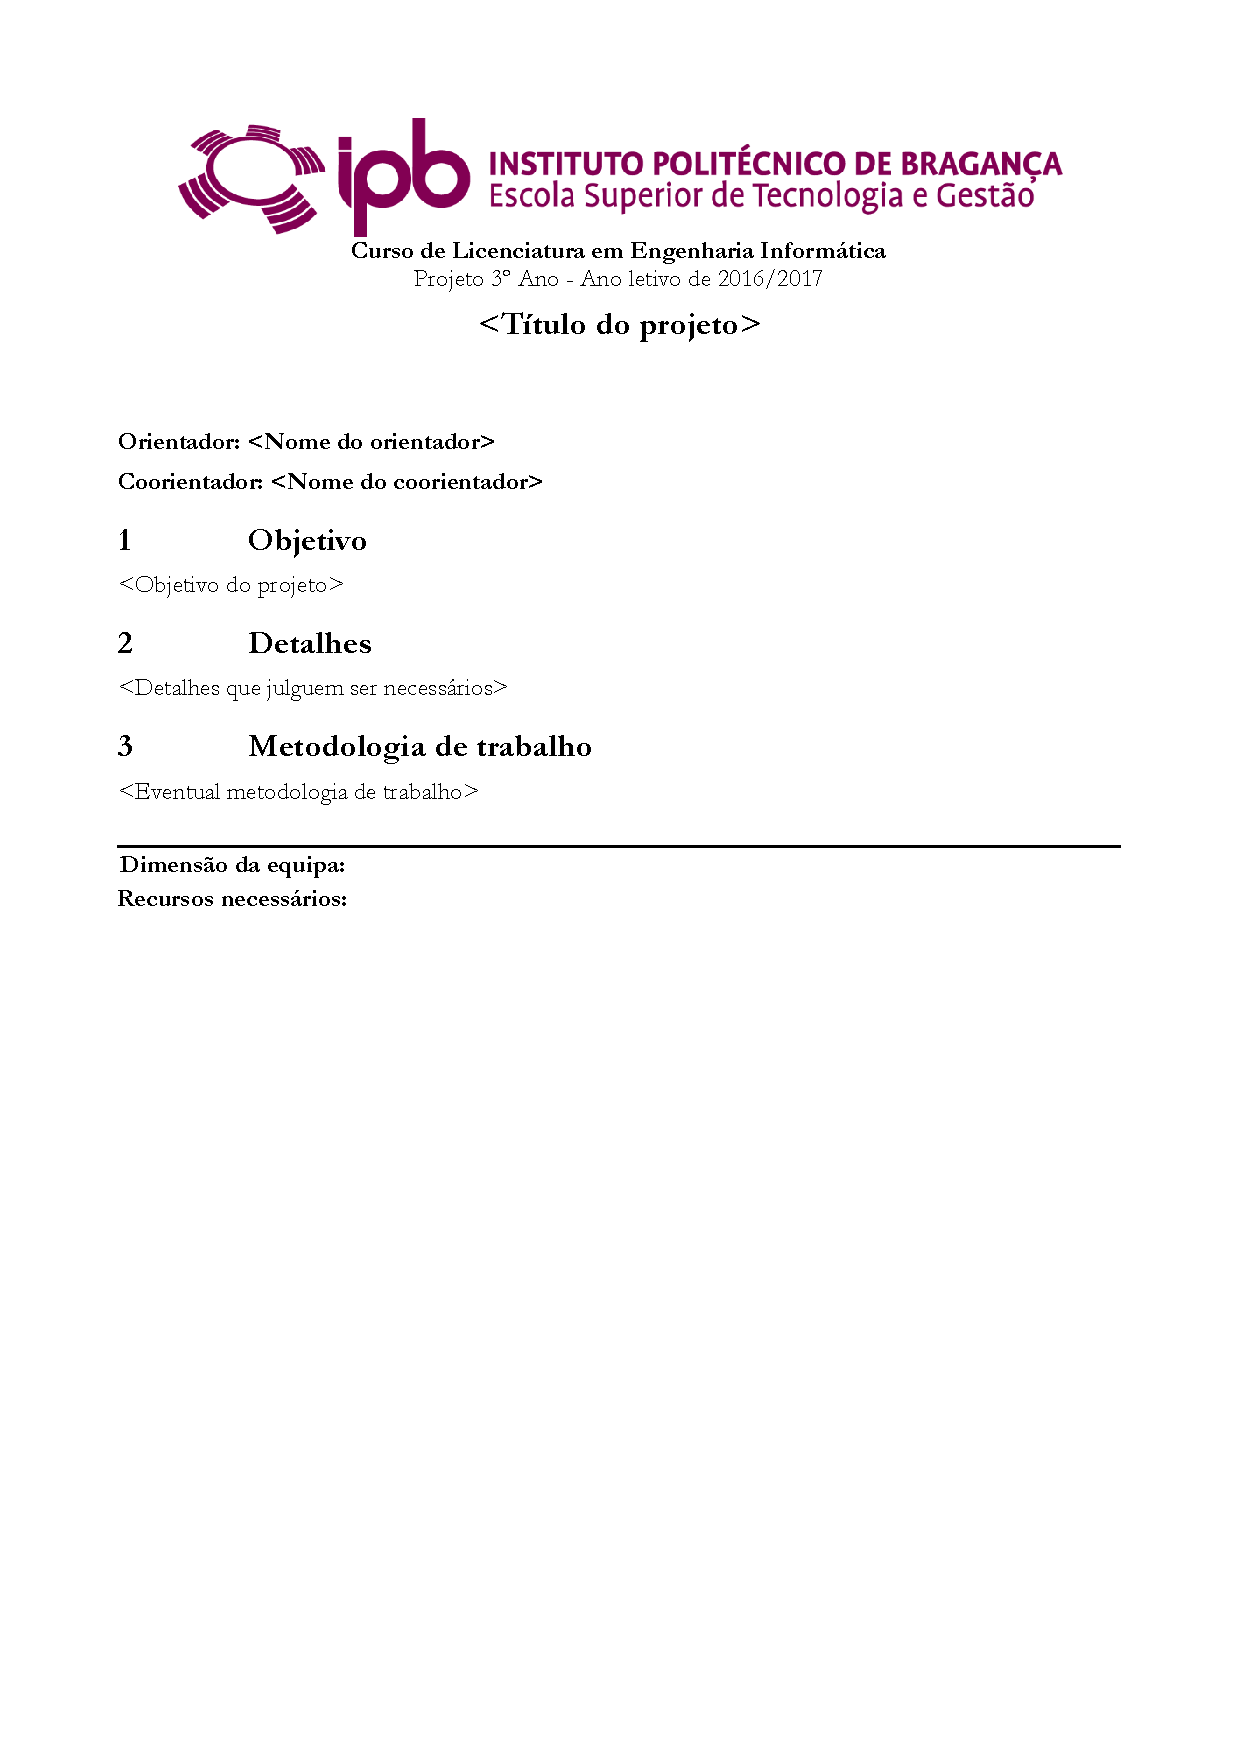
\includegraphics{etc/PropostaProjeto.pdf}
\end{figure}
\chapter{Outro(s) Apêndice(s)}
\label{apendice2}

Listagens de código fonte, texto/imagens produzidos por testes complementares, etc.


\end{document}
